\section{Conception}

\subsection{Délimitation fonctionnelle}

La section suivante est un rappel de la délimitation du circuit à concevoir. Celle-ci présente le contrôleur d'interruptions d'un point de vue extérieur avec les 6 relations définies précédemment.

\begin{figure}[H]
	\centering
	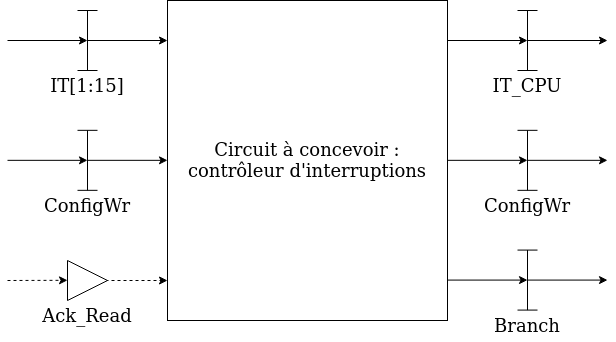
\includegraphics[width=0.6\linewidth]{figure/delimitation_fonctionnelle.png}
	\caption{Délimitation fonctionnelle du contrôleur d'interruptions}
	\label{fig:delimitation_fonctionnelle}
\end{figure}

Il s'agira par la suite de se placer dans un point de vue interne afin de présenter les différents blocs composant le contrôleur d'interruptions avec ses relations internes. 

\subsection{Décomposition fonctionnelle et introduction des interfaces}

La figure ci-dessous présente le circuit interne observé de l'intérieur avec l'introduction des signaux physiques du circuit. Il existe deux blocs nommés \texttt{Interface} et \texttt{Traitement}. 

\begin{figure}[H]
	\centering
	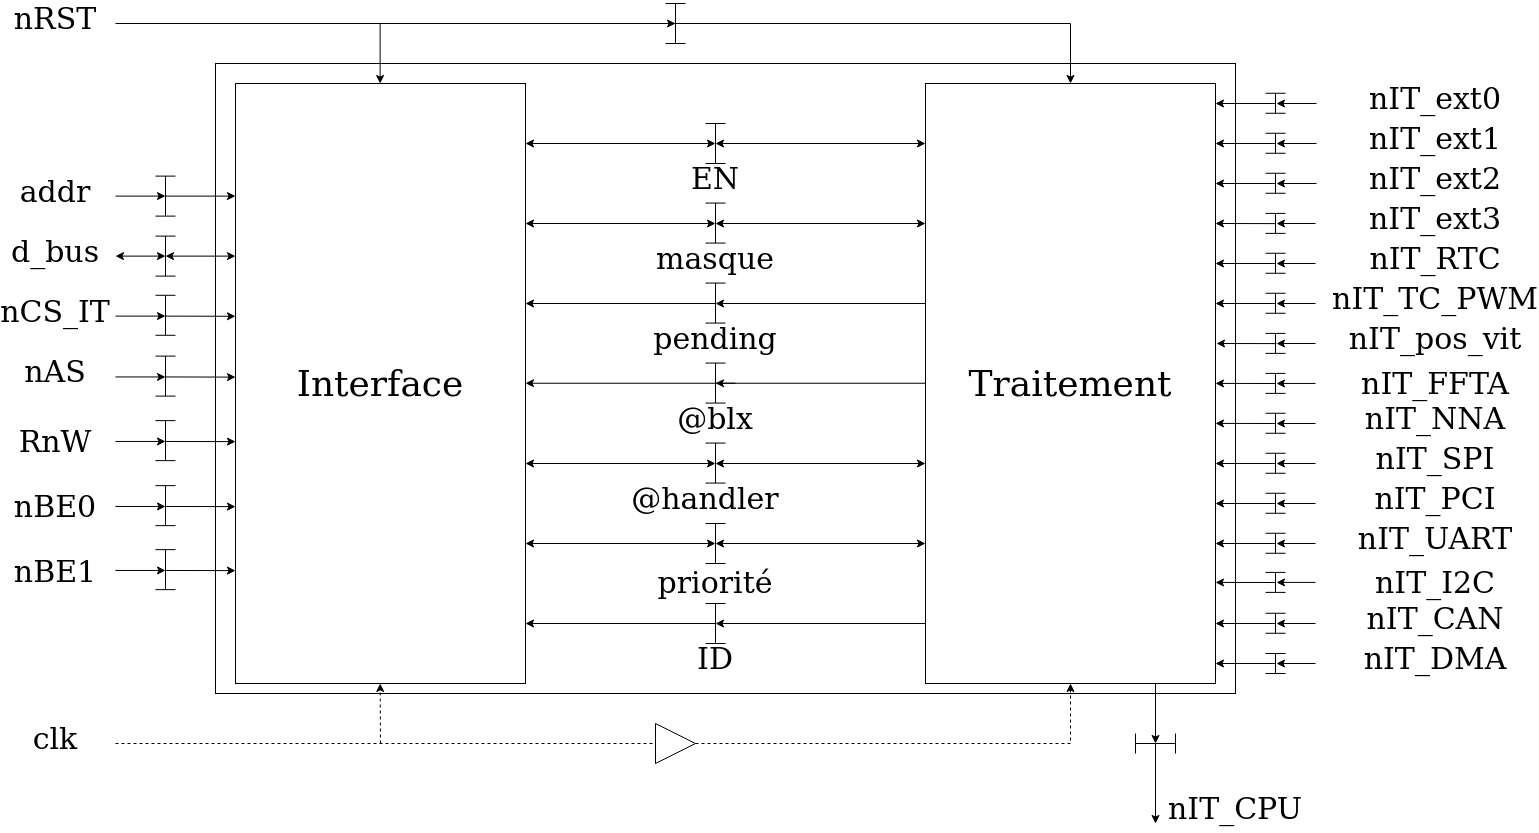
\includegraphics[width=1\linewidth]{figure/decomposition_fonctionnelle.png}
	\caption{Décomposition fonctionnelle et introduction des interfaces}
	\label{fig:decomposition_fonctionnelle}
\end{figure}

Le bloc \texttt{Traitement} est chargé de signaler le CPU d'une interruption à traiter à la suite de multiples opérations (traitement des priorités, opération de masquage, mise en suspens). Le bloc \texttt{Interface} permet de faire la jonction entre les signaux de contrôle et bus du système à microprocesseur et l'IP à concevoir. 

\newpage

\subsection{Raffinage du bloc \texttt{Interface}}

La section suivante présente un raffinage, c'est-à-dire de réaliser une seconde décomposition en se plaçant à l'intérieur du bloc \texttt{Interface}. Ce bloc est composé de \texttt{Interface\_Write} et \texttt{Interface\_Read}. 

\begin{figure}[H]
	\centering
	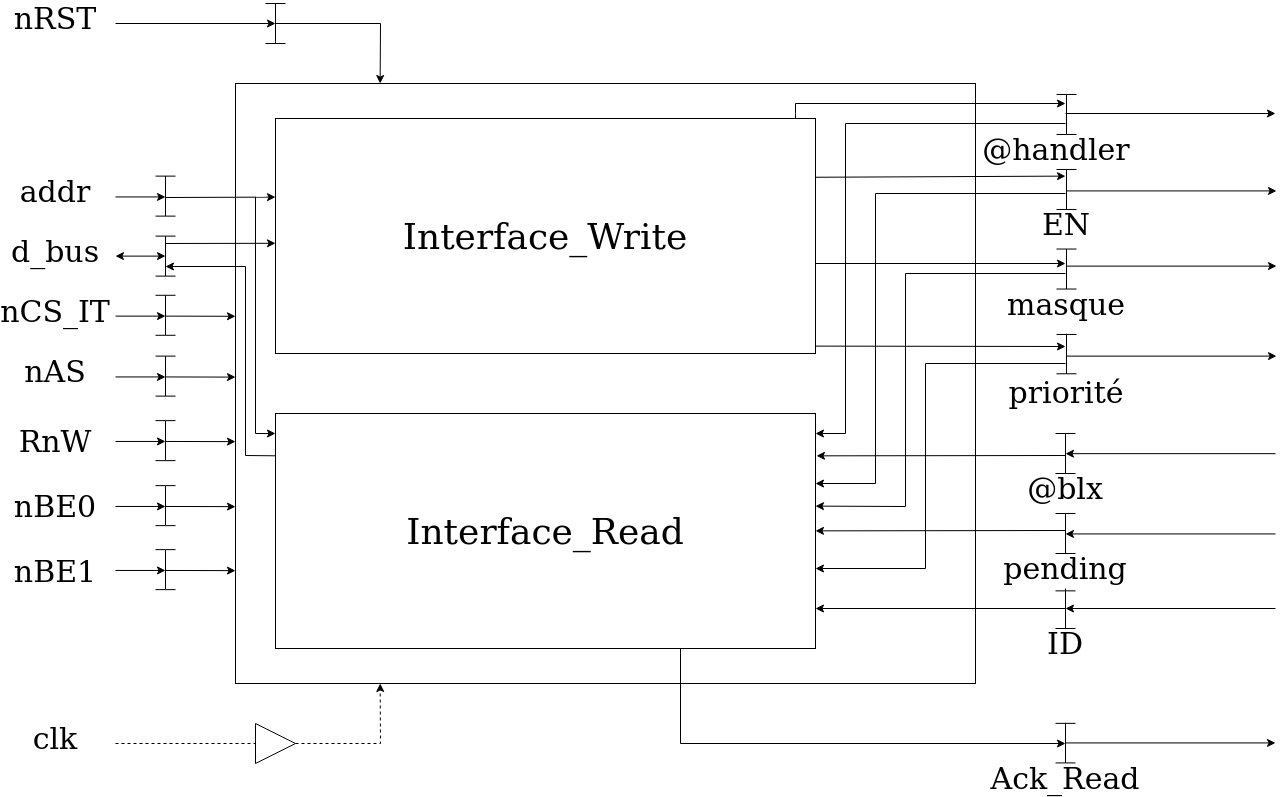
\includegraphics[width=0.9\linewidth]{figure/raffinage_interface.png}
	\caption{Raffinage et décomposition du bloc \texttt{Interface}}
	\label{fig:raffinage_interface}
\end{figure}

Cette décomposition en bloc hiérarchique permet de mettre en lumière deux fonctions du bloc \texttt{Interface}. Celui-ci peut écrire dans les registres du contrôleur d'interruptions par le biais du bloc \texttt{Interface\_Write} et les lire avec \texttt{Interface\_Read}.

\subsection{Raffinage du bloc \texttt{Traitement}}

\newpage

\subsection{Écriture des algorithmes}

\subsubsection{Algorithme \texttt{Interface\_Write}}

\subsubsection{Algorithme \texttt{Interface\_Read}}